\section{Grassmann tensor renormalization group}
\label{sec:GTRG}

The current Grassmann tensor network can be evaluated by coarse-graining algorithms 
with a truncation of degrees of freedom, 
such as the original Levin-Nave TRG \cite{Levin:2006jai} 
and some variations of the TRG \cite{PhysRevB.86.045139,Adachi:2019paf,Lan:2019stu,Kadoh:2019kqk}. 
In this section, we consider the higher-order TRG (HOTRG) \cite{PhysRevB.86.045139} applicable to any dimensional lattices 
for a Grassmann tensor network. 
%Thanks to the correspondence in Table~\ref{tab:correspondence}, 



\begin{figure}[htbp]
	\centering
	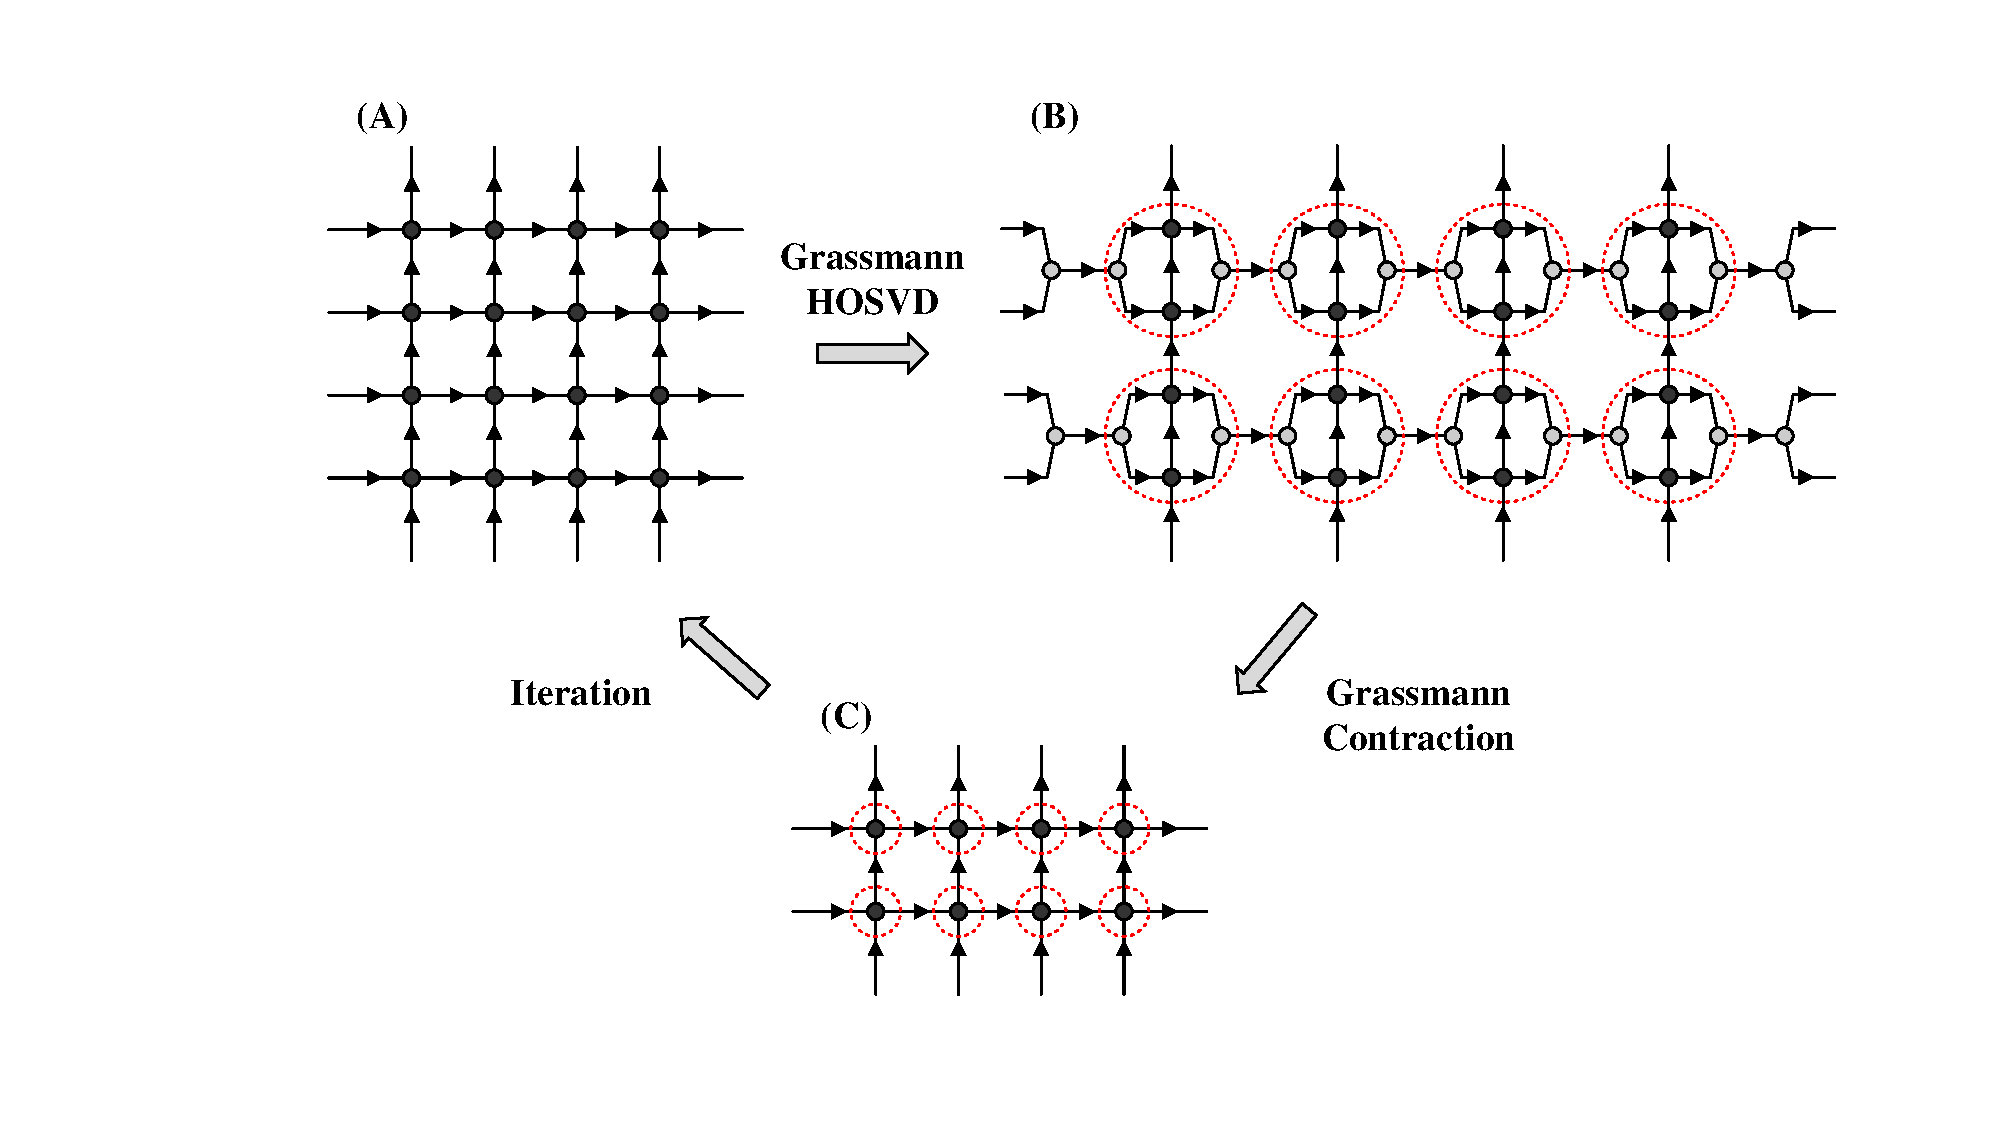
\includegraphics[width=1.\hsize]{ghotrg.pdf}
	\caption{Schematic picture of the Grassmann HOTRG. 
   (A) Grassmann tensor network in two dimensions. 
   (B) Grassmann isometries are inserted in the whole network. (C) Tensor network is renormalized so that 
    the lattice size is reduced by a factor of 2.}
	\label{fig:ghotrg}
\end{figure}

Let us consider a two dimensional case as an example. 
The Grassmann tensor network is made of a $4K$-rank Grassmann tensor, 
which is identified as the Grassmann tensor $\mathcal{T}_{XY\bar{Y} \bar{X}}$ 
of rank four with respect to $K$ component indices $X,\bar{X},Y,\bar{Y}$. 
Hereafter we count the rank of a Grassmann tensor in terms of $K$ component index.
We assume that $X$ and $Y$ live on the links $(n,n+\hat{\mu})$ for $\mu=1,2$, respectively 
and $\bar{X}$ and $\bar{Y}$ live on the links $(n,n-\hat{\mu})$ for $\mu=1,2$, respectively. 
In the initial Grassmann tensor network, $K=N$ which is the number of 
components in the original fermion field. 



Fig.~\ref{fig:ghotrg} schematically illustrates the algorithm of the current {\it Grassmann HOTRG}, 
which employs the higher-order singular value decomposition (HOSVD) for the coefficient tensor of
\begin{align}
\label{eq:M_HOTRG}
	\mathcal{M}_{X_{1}X_{2} Y \bar{Y}\bar{X}_{2}\bar{X}_{1}} = 
\int\diff\bar{\Xi}\diff\Xi~\e^{-\bar{\Xi}\Xi} 
\mathcal{T}_{X_{2}\Xi\bar{Y}\bar{X}_{2}} \mathcal{T}_{X_{1}Y\bar{\Xi}\bar{X}_{1}}.
\end{align}
$\mathcal{M}$ is identified as a Grassmann tensor of rank $6$, 
and the coefficient tensor $M$ which is read from Eq.~(\ref{eq:M_HOTRG}) 
is given by a contraction of coefficient tensor $T$ with some sign factors.

We can decompose $\mathcal{M}$ in a formal way,
\begin{align}
\label{eq:ghosvd}
	\mathcal{M}_{X_{1}X_{2}Y\bar{Y}\bar{X}_{2}\bar{X}_{1}}
=\left(\prod_{k=1}^{4}\int\diff\bar{\Xi}_{k}\diff\Xi_{k}~\e^{-\bar{\Xi}_{k}\Xi_{k}}\right) 
\mathcal{U}^{A}_{X_{1}X_{2}\Xi_{1}}\mathcal{U}^{B}_{Y\Xi_{2}}\mathcal{U}^{C}_{\bar{Y}\Xi_{3}} 
\mathcal{U}^{D}_{\bar{X}_{2}\bar{X}_{1}\Xi_{4}}\mathcal{S}_{\bar{\Xi}_{4}\bar{\Xi}_{3}\bar{\Xi}_{2}\bar{\Xi}_{1}}.
\end{align}
This decomposition is referred to as the {\it Grassmann HOSVD}, which is equivalent to the HOSVD 
for the coefficient tensor $M$. The Grassmann HOSVD gives us a {\it Grassmann isometry},
\begin{align}
\label{eq:isometry}
	\int\diff\bar{\Phi}\diff\Phi~\e^{-\bar{\Phi}\Phi}\mathcal{U}_{\bar{X}_{2}\bar{X}_{1}\Phi}\mathcal{U}_{\bar{\Phi} X_{1} X_{2}},
\end{align}
which is inserted into the Grassmann tensor network to truncate the bond degrees of 
freedom (Fig.~\ref{fig:ghotrg}(B)). $\mathcal{U}$ is chosen from $\mathcal{U}^{A}$ and $\mathcal{U}^{D}$ in 
Eq.~\eqref{eq:ghosvd}, following the algorithm of the HOTRG \cite{PhysRevB.86.045139}. 
Formally, $\Phi$ and $\bar{\Phi}$ in Eq.~\eqref{eq:isometry} are $(k+1)$-component 
Grassmann numbers, where $k$ is an integer such that $2^{k}<D<2^{k+1}$ with $D$ 
the bond dimension. However, a decimal numeral system defined in
 Ref.~\cite{Kadoh} (or see Appendix~\ref{sec:truncation}) allows us just 
to pick up $D^{2}\times D$ elements in the coefficient tensor in $\mathcal{U}$. 
This is practically useful to implement the current Grassmann HOTRG. 

Then, the coarse-graining renormalization is accomplished by the Grassmann contraction,
\begin{align}
	\mathcal{T}'_{X Y\bar{Y}\bar{X}}=\left(\prod_{i=1}^{2}\int\diff\bar{\Phi}_{i}
\diff\Phi_{i}~\e^{-\bar{\Phi}_{i}\Phi_{i}}\int\diff\bar{\Phi}'_{i}\diff\Phi'_{i}~\e^{-\bar{\Phi}'_{i}\Phi'_{i}}\right)
\mathcal{U}_{\bar{\Phi}_{2}\bar{\Phi}_{1}X}
\mathcal{M}_{\Phi_{1}\Phi_{2}Y\bar{Y}\bar{\Phi}'_{2}\bar{\Phi}'_{1}}\mathcal{U}_{\bar{X}\Phi'_{1}\Phi'_{2}}.
\end{align}
Iterating the above procedure, we can evaluate $Z$ by
\begin{align}
\label{eq:periodic}
	Z=\int\diff\bar{X}\diff X \e^{-\bar{X} X }\int\diff\bar{Y}\diff Y\e^{-\bar{Y} Y}\mathcal{T}_{X Y\bar{Y}\bar{X}}
\end{align}
with the periodic boundary condition. \footnote{If one imposes the anti-periodic boundary condition in $2$-direction, 
the multi Grassmann number in $\mathcal{T}$ on the link $(n,n+\hat{\mu})$, say $Y$, 
should be replaced by $-Y$ before carry out the integration in Eq.~\eqref{eq:periodic}}

We examine the above Grassmann HOTRG by benchmarking with the one-flavor colorless free 
Wilson fermion on a square lattice. We assume the anti-periodic boundary condition in $2$-direction. 
This free lattice fermion theory has been employed to test the efficiency of conventional 
Grassmann TRGs~\cite{Takeda:2014vwa,Sakai:2017jwp}.  
The initial tensor is given by Eq.(\ref{eq:Gtensor}) derived as a formula in the previous section. The explicit form is shown in Appendix \ref{sec:wilson}. 

Fig.~\ref{fig:l2} shows the free energy per site against the mass $M$ on $2\times2$ 
lattice with $D=16$. With the choice of $D\ge16$, the calculation by the current 
Grassmann HOTRG agrees with the exact results up to the machine precision. 
This situation is completely same with the conventional Grassmann HOTRG~\cite{Sakai:2017jwp}. 

Fig.~\ref{fig:delta} plots the relative error of the free energy on $1024\times1024$ lattice, defined by
\begin{align}
	\delta=\left|\frac{\ln Z(L=1024,D)-\ln Z_{\mathrm{exact}}(L=1024)}{\ln Z_{\mathrm{exact}}(L=1024)}\right|.
\end{align}
It is confirmed that the current Grassmann HOTRG has achieved the same accuracy with the conventional 
one both for massless and massive fermions. Hence, the current tensor network formulation enables us 
to study the lattice fermion theory with the TRG approach.

\begin{figure}[htbp]
	\centering
	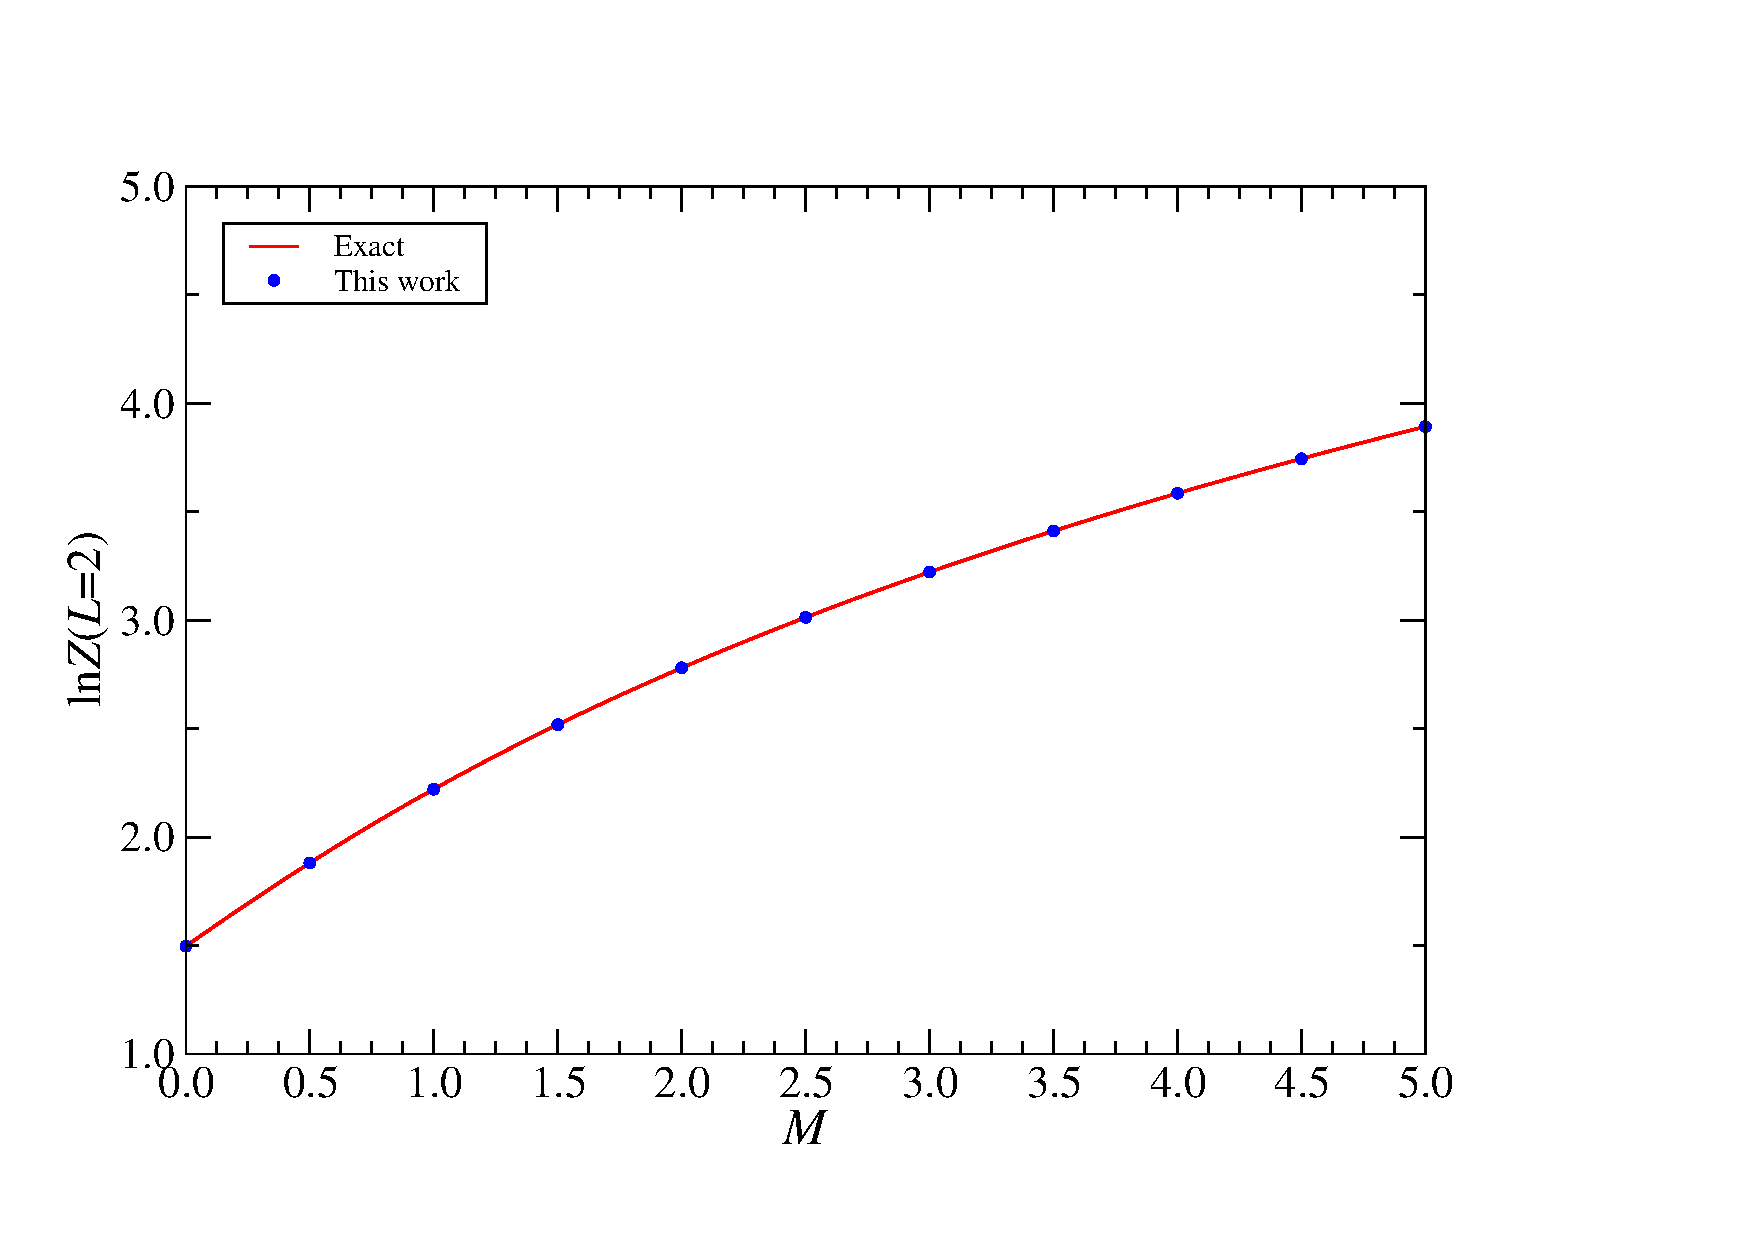
\includegraphics[width=.8\hsize]{l2.pdf}
	\caption{Free energy density for the free Wilson fermions against 
the mass $M$ on $2\times2$ lattice with $D=16$. It agrees with the exact values up to the machine precision. }
	\label{fig:l2}
\end{figure}


\begin{figure}[htbp]
	\centering
	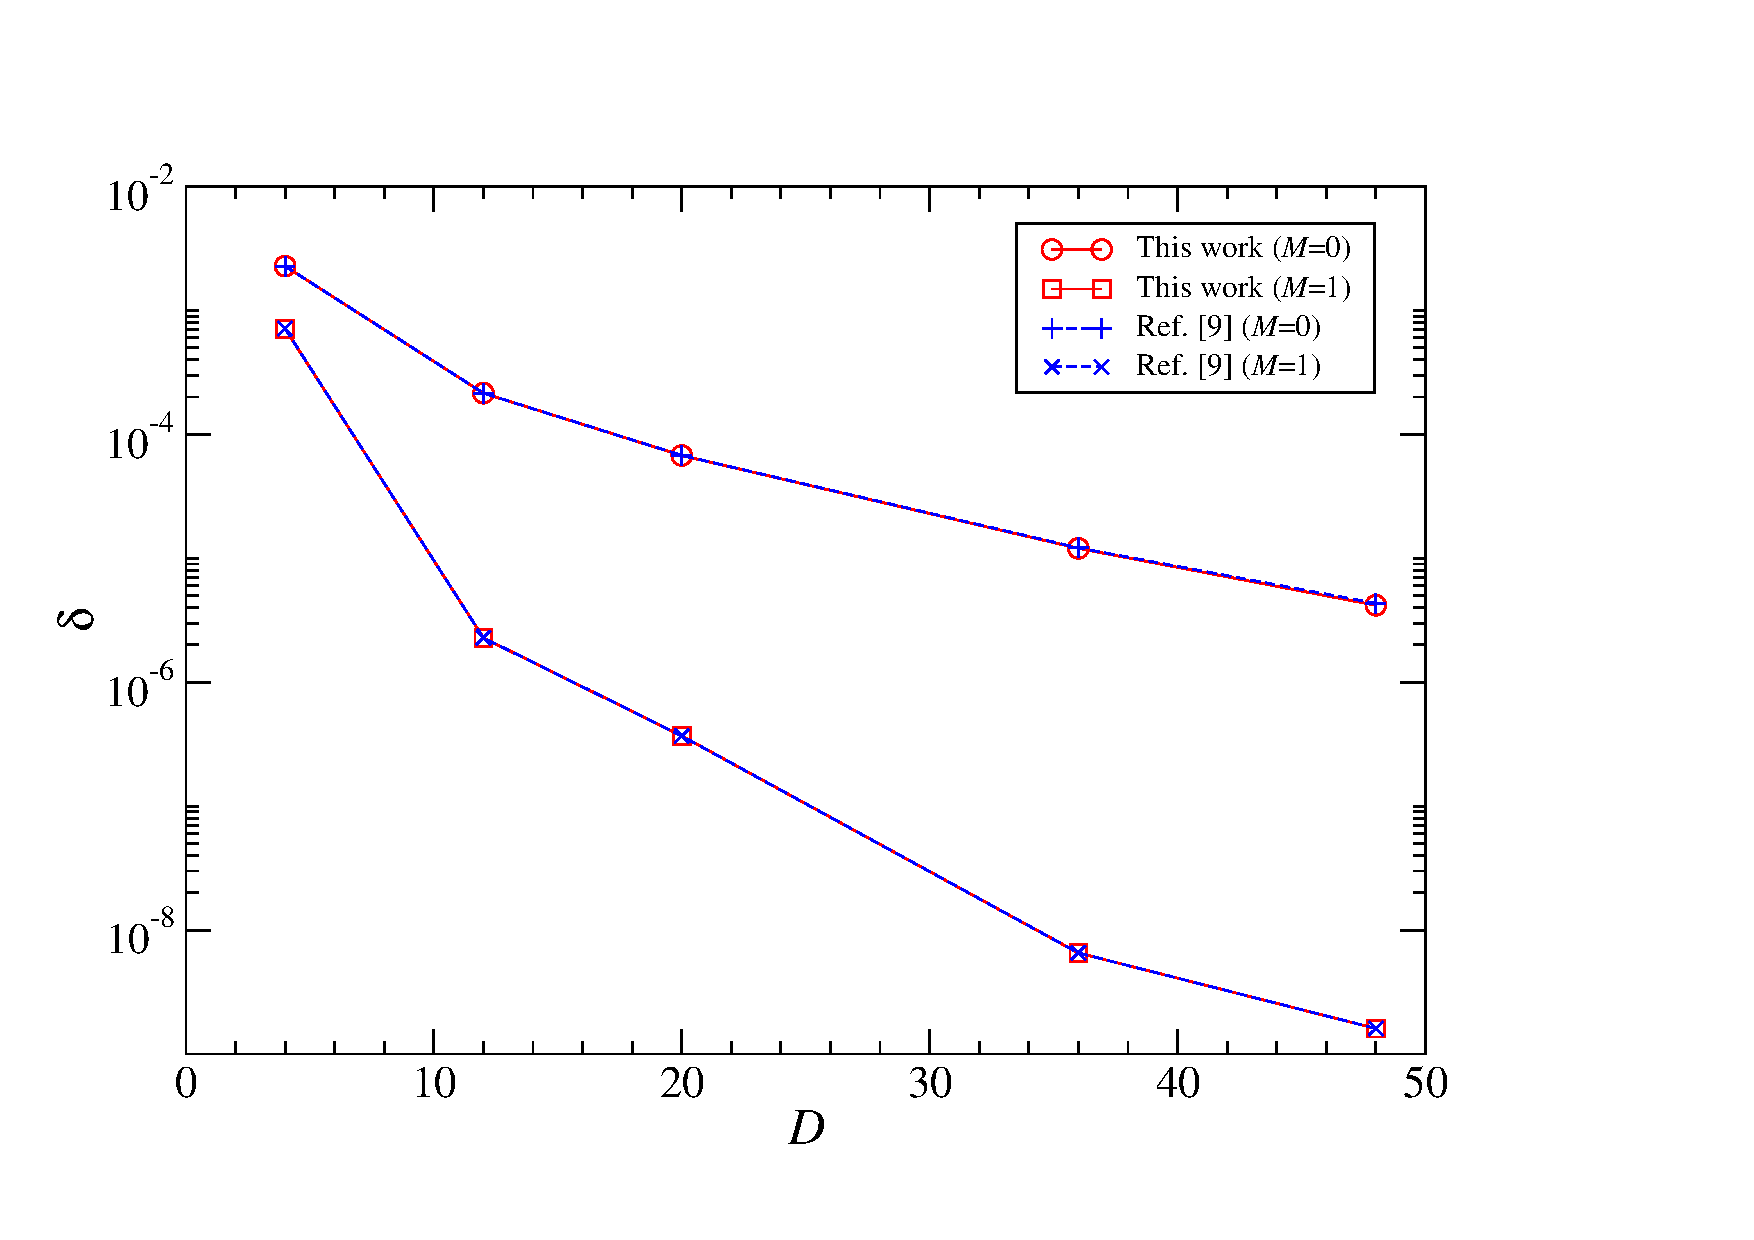
\includegraphics[width=.8\hsize]{select_delta.pdf}
	\caption{Relative error of the free energy on $1024\times1024$ lattice as a function of $D$. }
	\label{fig:delta}
\end{figure}














